\documentclass{article}

%other packages
\usepackage[a4paper]{geometry}
\usepackage{longtable}
\usepackage{wrapfig}
\setlength\parindent{0pt}
\usepackage{enumitem}
\usepackage[table,dvipsnames]{xcolor}
\usepackage{polynom}
\def\scaleint#1{\vcenter{\hbox{\scaleto[3ex]{\displaystyle\int}{#1}}}}
\usepackage{array}
\newcolumntype{C}{>{{}}c<{{}}} % for '+' and '-' symbols
\newcolumntype{R}{>{\displaystyle}r} % automatic display-style math mode 
\usepackage{tabularray}
\usepackage{dcolumn,tabularx,booktabs}
\usepackage[most]{tcolorbox}
%\graphicspath{ {C:/Users/twill/OneDrive/Desktop/Eliason/Diagrams} }

%maths
\usepackage{mathtools}
\usepackage{amsmath}
\usepackage{amssymb}
\usepackage{amsfonts}
\usepackage{autobreak}

%tikzpicture
\usepackage{tikz}
\usepackage{scalerel}
\usepackage{pict2e}
\usepackage{tkz-euclide}
\usepackage{tikz-3dplot}
\usetikzlibrary{calc}
\usetikzlibrary{patterns,arrows.meta}
\usetikzlibrary{shadows}
\usetikzlibrary{external}
\usetikzlibrary{decorations.pathreplacing,angles,quotes}

%pgfplots
\usepackage{pgfplots}
\pgfplotsset{compat=1.18}
\usepgfplotslibrary{statistics}
\usepgfplotslibrary{fillbetween}

\pgfplotsset{
    standard/.style={
    axis line style = thick,
    trig format=deg,
    enlargelimits,
    axis x line=middle,
    axis y line=middle,
    enlarge x limits=0.15,
    enlarge y limits=0.15,
    every axis x label/.style={at={(current axis.right of origin)},anchor=north west},
    every axis y label/.style={at={(current axis.above origin)},anchor=south east}
    }
}

\begin{document}

Math 115, 20 March 2024
\hrule

\vspace{10pt}

We first considered the following integral;

\[I_1=\int_1^\infty\frac{x^2+3x+5}{x^{5/2}+x^2-3x+4}\ dx\]

the integrand is similar to the quotient of the dominating terms of the numerator and denominator as the variable becomes unbounded,

\[f(x)\sim\frac{x^2}{x^{5/2}}=\frac{1}{\sqrt{x}}\]

meaning:

\[\lim_{x\to\infty}f(x)\div\frac{1}{\sqrt{x}}=1\]

\[\therefore I_1\mbox{ diverges by comparison.}\]

We then considered this integral;

\[\int\limits_0^1\ln x\ dx=(x=e^t)=\int\limits_{-\infty}^0te^t\ dx=(t=-u)=\int\limits_\infty^0ue^{-u}\ du\]

Then we looked at the Riemann Sum in general:

\begin{center}
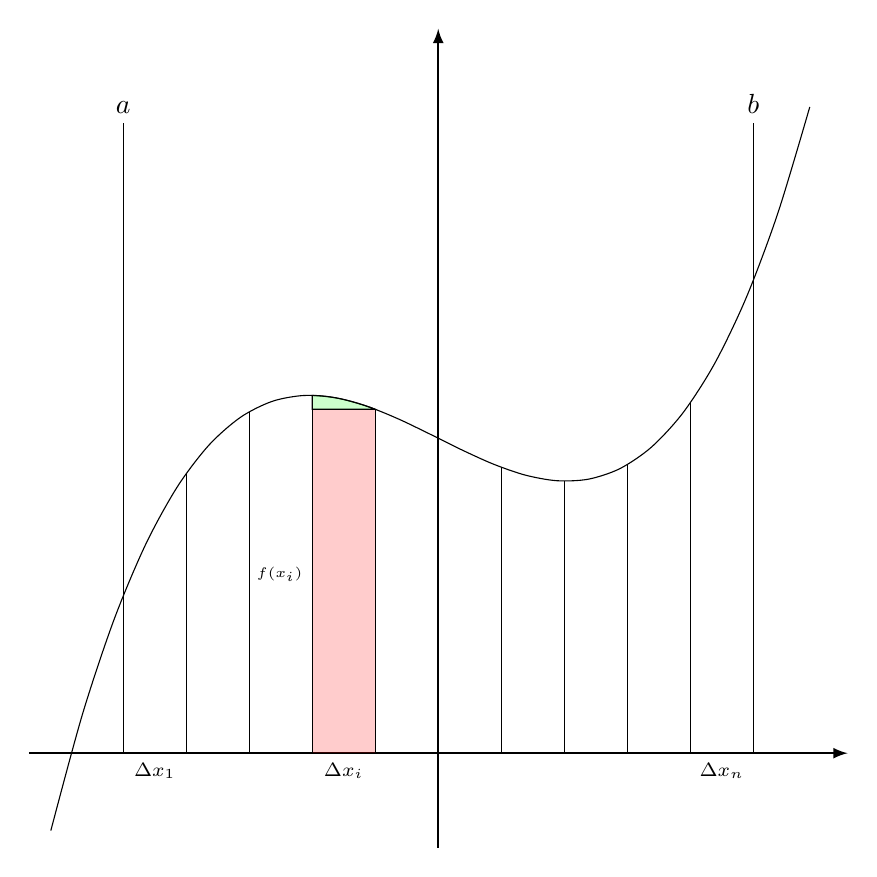
\begin{tikzpicture}[scale=4]
\draw[thick,-latex] (-1.3,0) -- (1.3,0);
\draw[thick,-latex] (0,-0.3) -- (0,2.3);
\draw[domain=-1.23:1.18,smooth,variable=\t]
  plot (\t,\t*\t*\t-0.5*\t+1,0);
\draw[] (-1,0) -- (-1,2) node[pos=1,above]{$a$};
\draw[] (1,0) -- (1,2) node[pos=1,above]{$b$};
\foreach \x in {-0.8,-0.6,...,0.8}{
\draw[] (\x,0) -- (\x,\x*\x*\x-0.5*\x+1);}
\path[] (-0.4,0) -- (-0.4,{-0.4*0.4*0.4+0.5*0.4+1}) node[pos=0.5,left]{$\scriptscriptstyle f(x_i)$};
\draw[fill=green, fill opacity=0.2, variable=\x,domain=-0.4:-0.2] (-0.4,{-0.4*0.4*0.4+0.5*0.4+1}) -- plot ({\x}, {\x*\x*\x-0.5*\x+1}) -- (-0.2,{-0.2*0.2*0.2+0.5*0.2+1}) -- (-0.4,{-0.2*0.2*0.2+0.5*0.2+1}) -- cycle;
\draw[fill=red, fill opacity=0.2, variable=\x,domain=-0.4:-0.2] (-0.4,0) -- (-0.4,{-0.2*0.2*0.2+0.5*0.2+1}) -- (-0.2,{-0.2*0.2*0.2+0.5*0.2+1}) -- (-0.2,0) -- cycle;
\node[below] at (-0.9,0) {$\scriptstyle \Delta x_1$};
\node[below] at (-0.3,0) {$\scriptstyle \Delta x_i$};
\node[below] at (0.9,0) {$\scriptstyle \Delta x_n$};
\end{tikzpicture}
\end{center}

This is just a list of each important part; for instance, the components of the area differential and the segment length are listed.

\[\Delta x_i=\frac{1}{n}(b-a);\ \Delta \color{red}A_i\color{black}\cong f(x_i)\Delta x_i;\ \Delta\color{green}A_i\color{black}=\Delta x_i\Delta h;\ A_{tot}=\sum_{i=1}^\infty f(x_i)\Delta x_i\]

The total area equals the area of the rectange and the curvilinear triangle on top of it. The rectangle has an explicit formula, and the curvilinear triangle can ignored doe to a higher order correction.

\[\Delta A_i=\Delta\color{red}A_i\color{black}+\Delta\color{green}A_i\color{black}=f(x_i)\Delta x+\ a\ higher\ order\ correction\]

This lets us express the integral in terms of simple rectangles.

\[\therefore f(x)\Delta x=\ dA(x)\implies A=\int_a^b\ dA(x)=\int_a^bf(x)\ dx\]

And this is consistent with treating the area differential as an infinitesimal difference:

\[dF(x)=F(x+dx)-F(x)=F^\prime(x)\ dx+o(dx)\quad\mbox{ where }\quad o(dx)=\mbox{ higher order correction}\]

That is,

\[o(h):\lim_{h\to0}\frac{O(h)}{h}=0\]

\newpage
Remember that areas under the axis are negative,

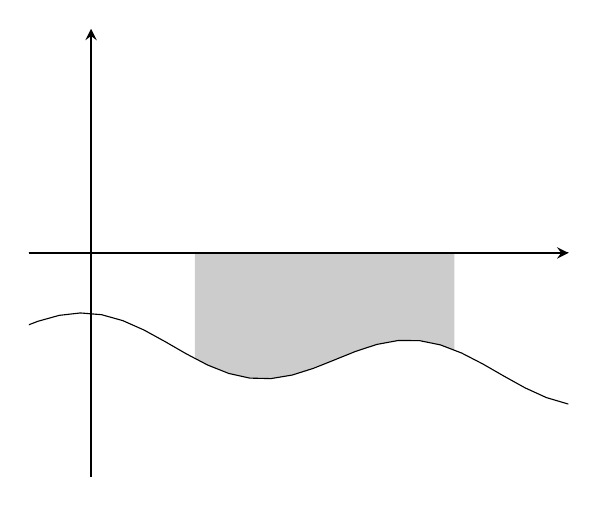
\begin{tikzpicture}
\begin{axis}[
standard,
xmin=0, xmax=4,
ymin=-2, ymax=2,
xtick={\empty}, ytick={\empty}]
\addplot[samples=50, name path=G] {0};
\addplot[samples=50, name path=F] {-0.1*x-1+0.3*cos(deg(2*x))};
\addplot[fill=black, fill opacity=0.2] fill between [of=F and G, soft clip={domain=1:3.5}];
\end{axis}
\end{tikzpicture}

and the area between two curves that intersect each other is doneby taking each region individually, as the order you subtract them in depends on which one is on top

\begin{tikzpicture}
\begin{axis}[
standard,
xmin=0, xmax=4,
ymin=-1, ymax=1,
xtick={\empty}, ytick={\empty}]
\addplot[samples=50] {-0.1*(x-2)+0.5+0.3*cos(deg((x-2)/2))};
\addplot[samples=50] {0.1*(x-2)+0.5+0.3*cos(deg((x-2)/1.5))};
\end{axis}
\end{tikzpicture}








\end{document}
